\documentclass[english,hidelinks, 11 pt, class=report,crop=false]{standalone}
\usepackage[T1]{fontenc}
%\usepackage[utf8]{inputenc}
\usepackage{lmodern} % load a font with all the characters
\usepackage{geometry}
\geometry{verbose,paperwidth=16.1 cm, paperheight=24 cm, inner=2.3cm, outer=1.8 cm, bmargin=2cm, tmargin=1.8cm}
\setlength{\parindent}{0bp}
\usepackage{import}
\usepackage[subpreambles=false]{standalone}
\usepackage{amsmath}
\usepackage{amssymb}
\usepackage{esint}
\usepackage{babel}
\usepackage{tabu}
\makeatother
\makeatletter

\usepackage{titlesec}
\usepackage{ragged2e}
\RaggedRight
\raggedbottom
\frenchspacing

\usepackage{graphicx}
\usepackage{float}
\usepackage{subfig}
\usepackage{placeins}
\usepackage{cancel}
\usepackage{framed}
\usepackage{wrapfig}
\usepackage[subfigure]{tocloft}
\usepackage[font=footnotesize,labelfont=sl]{caption} % Figure caption
\usepackage{bm}
\usepackage[dvipsnames, table]{xcolor}
\definecolor{shadecolor}{rgb}{0.105469, 0.613281, 1}
\colorlet{shadecolor}{Emerald!15} 
\usepackage{icomma}
\makeatother
\usepackage[many]{tcolorbox}
\usepackage{multicol}
\usepackage{stackengine}

\usepackage{esvect} %For vectors with capital letters

% For tabular
\usepackage{array}
\usepackage{multirow}
\usepackage{longtable} %breakable table

% Ligningsreferanser
\usepackage{mathtools} % for mathclap
%\mathtoolsset{showonlyrefs}

% sections without numbering in toc
\newcommand\tsec[1]{\phantomsection \addcontentsline{toc}{section}{#1}
	\section*{#1}}

% index
\usepackage{imakeidx}
\makeindex[title=Indeks]

%Footnote:
\usepackage[bottom, hang, flushmargin]{footmisc}
\usepackage{perpage} 
\MakePerPage{footnote}
\addtolength{\footnotesep}{2mm}
\renewcommand{\thefootnote}{\arabic{footnote}}
\renewcommand\footnoterule{\rule{\linewidth}{0.4pt}}
\renewcommand{\thempfootnote}{\arabic{mpfootnote}}

%colors
\definecolor{c1}{cmyk}{0,0.5,1,0}
\definecolor{c2}{cmyk}{1,0.25,1,0}
\definecolor{n3}{cmyk}{1,0.,1,0}
\definecolor{neg}{cmyk}{1,0.,0.,0}


\newcommand{\nreq}[1]{
\begin{equation}
	#1
\end{equation}
}


% Equation comments
\newcommand{\cm}[1]{\llap{\color{blue} #1}}


\usepackage[inline]{enumitem}
\newcounter{rg}
\numberwithin{rg}{chapter}


\newcommand{\reg}[2][]{\begin{tcolorbox}[boxrule=0.3 mm,arc=0mm,colback=blue!3] {\refstepcounter{rg}\phantomsection \large \textbf{\therg \;#1} \vspace{5 pt}}\newline #2  \end{tcolorbox}\vspace{-5pt}}
\newcommand{\regdef}[2][]{\begin{tcolorbox}[boxrule=0.3 mm,arc=0mm,colback=blue!3] {\refstepcounter{rg}\phantomsection \large \textbf{\therg \;#1} \vspace{5 pt}}\newline #2  \end{tcolorbox}\vspace{-5pt}}
\newcommand{\words}[1]{\begin{tcolorbox}[boxrule=0.3 mm,arc=0mm,colback=teal!3] #1  \end{tcolorbox}\vspace{-5pt}}

\newcommand\alg[1]{\begin{align*} #1 \end{align*}}

\newcommand\eks[2][]{\begin{tcolorbox}[boxrule=0.3 mm,arc=0mm,enhanced jigsaw,breakable,colback=green!3] {\large \textbf{\ekstitle #1} \vspace{5 pt}\\} #2 \end{tcolorbox}\vspace{-5pt} }

\newcommand{\st}[1]{\begin{tcolorbox}[boxrule=0.0 mm,arc=0mm,enhanced jigsaw,breakable,colback=yellow!12]{ #1} \end{tcolorbox}}

\newcommand{\spr}[1]{\begin{tcolorbox}[boxrule=0.3 mm,arc=0mm,enhanced jigsaw,breakable,colback=yellow!7] {\large \textbf{\sprtitle} \vspace{5 pt}\\} #1 \end{tcolorbox}\vspace{-5pt} }

\newcommand{\sym}[1]{\colorbox{blue!15}{#1}}

\newcommand{\info}[2]{\begin{tcolorbox}[boxrule=0.3 mm,arc=0mm,enhanced jigsaw,breakable,colback=cyan!6] {\large \textbf{#1} \vspace{5 pt}\\} #2 \end{tcolorbox}\vspace{-5pt} }

\newcommand\algv[1]{\vspace{-11 pt}\begin{align*} #1 \end{align*}}

\newcommand{\regv}{\vspace{5pt}}
\newcommand{\mer}{\textsl{\note}: }
\newcommand{\mers}[1]{{\footnotesize \mer #1}}
\newcommand\vsk{\vspace{11pt}}
\newcommand{\tbs}{\vspace{5pt}}
\newcommand\vs{\vspace{-11pt}}
\newcommand\vsb{\vspace{-16pt}}
\newcommand\br{\\[5 pt]}
\newcommand{\figp}[1]{../fig/#1}
\newcommand\algvv[1]{\vs\vs\begin{align*} #1 \end{align*}}
\newcommand{\y}[1]{$ {#1} $}
\newcommand{\os}{\\[5 pt]}
\newcommand{\prbxl}[2]{
\parbox[l][][l]{#1\linewidth}{#2
	}}
\newcommand{\prbxr}[2]{\parbox[r][][l]{#1\linewidth}{
		\setlength{\abovedisplayskip}{5pt}
		\setlength{\belowdisplayskip}{5pt}	
		\setlength{\abovedisplayshortskip}{0pt}
		\setlength{\belowdisplayshortskip}{0pt} 
		\begin{shaded}
			\footnotesize	#2 \end{shaded}}}
\newcommand{\fgbxr}[2]{
	\parbox[r][][l]{#1\linewidth}{#2
}}		

\renewcommand{\cfttoctitlefont}{\Large\bfseries}
\setlength{\cftaftertoctitleskip}{0 pt}
\setlength{\cftbeforetoctitleskip}{0 pt}

\newcommand{\bs}{\\[3pt]}
\newcommand{\vn}{\\[6pt]}
\newcommand{\fig}[1]{\begin{figure}[H]
		\centering
		\includegraphics[]{\figp{#1}}
\end{figure}}

\newcommand{\figc}[2]{\begin{figure}
		\centering
		\includegraphics[]{\figp{#1}}
		\caption{#2}
\end{figure}}
\newcommand{\arc}[1]{{
		\setbox9=\hbox{#1}%
		\ooalign{\resizebox{\wd9}{\height}{\texttoptiebar{\phantom{A}}}\cr\textit{#1}}}}

\newcommand{\sectionbreak}{\clearpage} % New page on each section

\newcommand{\nn}[1]{
\begin{equation*}
	#1
\end{equation*}
}

\newcommand{\enh}[1]{\,\textrm{#1}}

%asin, atan, acos
\DeclareMathOperator{\atan}{atan}
\DeclareMathOperator{\acos}{acos}
\DeclareMathOperator{\asin}{asin}

% Comments % old cm, ggb cm is new
%\newcommand{\cm}[1]{\llap{\color{blue} #1}}

%%%

\newcommand\fork[2]{\begin{tcolorbox}[boxrule=0.3 mm,arc=0mm,enhanced jigsaw,breakable,colback=yellow!7] {\large \textbf{#1 (\expl)} \vspace{5 pt}\\} #2 \end{tcolorbox}\vspace{-5pt} }
 
%colors
\newcommand{\colr}[1]{{\color{red} #1}}
\newcommand{\colb}[1]{{\color{blue} #1}}
\newcommand{\colo}[1]{{\color{orange} #1}}
\newcommand{\colc}[1]{{\color{cyan} #1}}
\definecolor{projectgreen}{cmyk}{100,0,100,0}
\newcommand{\colg}[1]{{\color{projectgreen} #1}}

% Methods
\newcommand{\metode}[2]{
	\textsl{#1} \\[-8pt]
	\rule{#2}{0.75pt}
}

%Opg
\newcommand{\abc}[1]{
	\begin{enumerate}[label=\alph*),leftmargin=18pt]
		#1
	\end{enumerate}
}
\newcommand{\abcs}[2]{
	\begin{enumerate}[label=\alph*),start=#1,leftmargin=18pt]
		#2
	\end{enumerate}
}
\newcommand{\abcn}[1]{
	\begin{enumerate}[label=\arabic*),leftmargin=18pt]
		#1
	\end{enumerate}
}
\newcommand{\abch}[1]{
	\hspace{-2pt}	\begin{enumerate*}[label=\alph*), itemjoin=\hspace{1cm}]
		#1
	\end{enumerate*}
}
\newcommand{\abchs}[2]{
	\hspace{-2pt}	\begin{enumerate*}[label=\alph*), itemjoin=\hspace{1cm}, start=#1]
		#2
	\end{enumerate*}
}

% Exercises


\newcounter{opg}
\numberwithin{opg}{section}

\newcounter{grub}
\numberwithin{opg}{section}
\newcommand{\op}[1]{\vspace{15pt} \refstepcounter{opg}\large \textbf{\color{blue}\theopg} \vspace{2 pt} \label{#1} \\}
\newcommand{\eksop}[2]{\vspace{15pt} \refstepcounter{opg}\large \textbf{\color{blue}\theopg} (#1) \vspace{2 pt} \label{#2} \\}

\newcommand{\nes}{\stepcounter{section}
	\setcounter{opg}{0}}
\newcommand{\opr}[1]{\vspace{3pt}\textbf{\ref{#1}}}
\newcommand{\oeks}[1]{\begin{tcolorbox}[boxrule=0.3 mm,arc=0mm,colback=white]
		\textit{\ekstitle: } #1	  
\end{tcolorbox}}
\newcommand\opgeks[2][]{\begin{tcolorbox}[boxrule=0.1 mm,arc=0mm,enhanced jigsaw,breakable,colback=white] {\footnotesize \textbf{\ekstitle #1} \\} \footnotesize #2 \end{tcolorbox}\vspace{-5pt} }


% tag exercises
\newcommand{\tagop}[1]{ 
{\small \color{Gray} #1} \os
}

% License
\newcommand{\lic}{
This book is part of the \net{https://sindrsh.github.io/openmathbooks/}{OpenMathBooks} project. OpenMathBooks © 2022 by Sindre Sogge Heggen is licensed under CC BY-NC-SA 4.0. To view a copy of this license, visit \net{http://creativecommons.org/licenses/by-nc-sa/4.0/}{http://creativecommons.org/licenses/by-nc-sa/4.0/}}

%referances
\newcommand{\net}[2]{{\color{blue}\href{#1}{#2}}}
\newcommand{\hrs}[2]{\hyperref[#1]{\color{blue}#2 \ref*{#1}}}
\newcommand{\refunnbr}[2]{\hyperref[#1]{\color{blue}#2}}


\newcommand{\openmath}{\net{https://sindrsh.github.io/openmathbooks/}{OpenMathBooks}}
\newcommand{\am}{\net{https://sindrsh.github.io/FirstPrinciplesOfMath/}{AM1}}
\newcommand{\mb}{\net{https://sindrsh.github.io/FirstPrinciplesOfMath/}{MB}}
\newcommand{\tmen}{\net{https://sindrsh.github.io/FirstPrinciplesOfMath/}{TM1}}
\newcommand{\tmto}{\net{https://sindrsh.github.io/FirstPrinciplesOfMath/}{TM2}}
\newcommand{\amto}{\net{https://sindrsh.github.io/FirstPrinciplesOfMath/}{AM2}}
\newcommand{\eksbm}{
\footnotesize
Dette er opppgaver som har blitt gitt ved sentralt utformet eksamen i Norge. Oppgavene er laget av Utdanningsdirektoratet. Forkortelser i parantes viser til følgende:
\begin{center}
	\begin{tabular}{c|c}
		E & Eksempeloppgave \\
		V/H & Eksamen fra vårsemesteret/høstsemesteret\\
		G/1P/1T/R1/R2 & Fag  \\
		XX & År 20XX \\
		D1/D2 & Del 1/Del 2
	\end{tabular}
\end{center}
Tekst og innhold kan her være noe endret i forhold til originalen.
}

%Excel og GGB:

\newcommand{\g}[1]{\begin{center} {\tt #1} \end{center}}
\newcommand{\gv}[1]{\begin{center} \vspace{-11 pt} {\tt #1}  \end{center}}
\newcommand{\cmds}[2]{{\tt #1}\\
	#2}

% outline word
\newcommand{\outl}[1]{{\boldmath \color{teal}\textbf{#1}}}
%line to seperate examples
\newcommand{\linje}{\rule{\linewidth}{1pt} }


%Vedlegg
\newcounter{vedl}
\newcounter{vedleq}
\renewcommand\thevedl{\Alph{vedl}}	
\newcommand{\nreqvd}{\refstepcounter{vedleq}\tag{\thevedl \thevedleq}}

%%% Writing code

\usepackage{listings}


\definecolor{codegreen}{rgb}{0,0.6,0}
\definecolor{codegray}{rgb}{0.5,0.5,0.5}
\definecolor{codepurple}{rgb}{0.58,0,0.82}
\definecolor{backcolour}{rgb}{0.95,0.95,0.92}

\newcommand{\pymet}[1]{{\ttfamily\color{magenta} #1}}
\newcommand{\pytype}[1]{{\ttfamily\color{codepurple} #1}}

\lstdefinestyle{mystyle}{
	backgroundcolor=\color{backcolour},   
	commentstyle=\color{codegreen},
	keywordstyle=\color{magenta},
	numberstyle=\tiny\color{codegray},
	stringstyle=\color{codepurple},
	basicstyle=\ttfamily\footnotesize,
	breakatwhitespace=false,         
	breaklines=true,                 
	captionpos=b,                    
	keepspaces=true,                 
	numbers=left,                    
	numbersep=5pt,                  
	showspaces=false,                
	showstringspaces=false,
	showtabs=false,                  
	tabsize=2,
	inputencoding=utf8,
	extendedchars=true,
	literate= {
		{å}{{\aa}}1 
		{æ}{{\ae}}1 
		{ø}{{\o}}1
	}
}

\lstset{style=mystyle}

\newcommand{\python}[1]{
\begin{tcolorbox}[boxrule=0.3 mm,arc=0mm,colback=white]
\lstinputlisting[language=Python]{#1}
\end{tcolorbox}}
\newcommand{\pythonut}[2]{
\begin{tcolorbox}[boxrule=0.3 mm,arc=0mm,colback=white]
\small 
%\textbf{Kode}
\lstinputlisting[language=Python]{#1}	
\vspace{11pt}
\textbf{Utdata} \\ \ttfamily
#2
\end{tcolorbox}}
%%%

%page number
%\usepackage{fancyhdr}
%\pagestyle{fancy}
%\fancyhf{}
%\renewcommand{\headrule}{}
%\fancyhead[RO, LE]{\thepage}

\usepackage{datetime2}
%%\usepackage{sansmathfonts} for dyslexia-friendly math
\usepackage[]{hyperref}




\begin{document}
\subsection*{Oppgave 1}	
\[ \int_{-1}^{1}x^3+2x\,dx = \left[\frac{1}{4}x^4+x^2\right]_{-1}^1 = 0 \]
Dette svart forteller at arealet avgrenset av grafen til $ x^3+2x $ og $ x $-aksen er like stort på begge sider av $ x $-aksen på intervallet $ [-1, 1] $.

\subsection*{Oppgave 2}
$ x $-verdiene til de to skjæringspunktene gjenkjenner vi som $ x=\frac{\pi}{4} $ og $ x=-\frac{3\pi}{4} $ (fordi da er $ \cos x =\sin x $). Da $ \cos x\geq \sin x $ for $ x\in\left[-\frac{3\pi}{4}, \frac{\pi}{4}\right] $, er arealet til det fargede området gitt som

\[ \int_{-\frac{3\pi}{4}}^{\frac{\pi}{4}} \cos x-\sin x \,dx =\Big[\sin x + \cos x\Big]_{-\frac{3\pi}{4}}^{\frac{\pi}{4}}=\frac{\sqrt{2}}{2}+\frac{\sqrt{2}}{2}-\left(-\frac{\sqrt{2}}{2}-\frac{\sqrt{2}}{2}\right)=2\sqrt{2} \]

\subsection*{Oppgave 3}
\abc{
	\item Da summen av den uendelige rekka er 8, og $ a_1=4 $, har vi av formelen for summen av en uendelig geometrisk rekke at
	\[ 8=\frac{4}{1-k} \] 
	Altså er $ k=\frac{1}{2} $, og dermed har vi av formelen for summen av en geometrisk rekke at
	\alg{
		S_4 = 4\cdot\frac{1-\left(\frac{1}{2}\right)^4}{1-\frac{1}{2}}=\frac{15}{2}
	}
	\item Den eksplisitte formelen for ledd $ i $ i en aritmetisk rekke er $ a_i = a_1+d(i-1) $, og dermed har vi at
	\[ a_1 +a_4 + a_7 = a_1 + (a_1+3d) + (a_1+6d)=3a_1+9d=3(a_1+3d)=3a_4 \]
	Altså er
	\algv{
		3a_4 &= 114 \\
		a_4 &= 38
	}
}
\newpage
\subsection*{Oppgave 4}
\abc{
\item Ut ifra koeffisientene foran $ x $, $ y $ og $ z $ i likningene til planet, har vi at $ [1, -2, 2] $ er en normalvektor til $ \alpha $. En parameterframstilling $ l $ for linja gjennom $ A $ som står normalt på planet $ \alpha $ er dermed gitt som
	\begin{equation}l: \left\lbrace{
		\begin{array}{lll}
			x= 4 + t   \\
			y= 2 + -2t    \\
			z= 2 + 2t 
		\end{array}
	}\right. 
\end{equation}
\item Vi bruker formelen for avstanden $ h $ mellom et punkt og et plan, og får at 
\[ h=\frac{\left|4+2(-2)+2\cdot2+1\right|}{\sqrt{1^2+(-2)+2^2}}=\frac{5}{3} \]
}
\newpage
\subsection*{Oppgave 5}
\abc{
\item Eleven ønsker å finne det samlede arealet avgrenset av grafen til $ f(x)=x^2-1 $ og $ x $-aksen på intervallet $ [-2, 2] $. Dette fordi eleven i skriptet
\begin{itemize}
	\item definerer nevnte funksjon og intervall.
	\item ved bruk av en for-løkke tilnærmer integralet $ \int_{-2}^{2}|f|\, dx $, som gir det nevnte arealet.
\end{itemize}
\item På intervallet $ [-2, 2] $ er $ f(x)=x^2-1 $ positiv når $ |x|>1 $ og negativ når $ |x|<1 $. Følgelig er
\[ \int_{-2}^{2}|f|\,dx = \int_{-2}^{-1} f\,dx + \int_{-1}^{1} -f\,dx+\int_{1}^{2}f\,dx \]
}
Vi har at 
\alg{
\int x^2-1 \, dx &= \frac{1}{3}x^3-x \br
\left[\frac{1}{3}x^3-x\right]_{-2}^{-1}&=-\frac{1}{3}+1-\left(-\frac{8}{3}+2\right)=\frac{4}{3} \br
-\left[\frac{1}{3}x^3-x\right]_{-1}^{1}&=-\frac{1}{3}+1+\left(-\frac{1}{3}+1\right)=\frac{4}{3} \br
\left[\frac{1}{3}x^3-x\right]_{1}^{2}&=\frac{8}{3}-2-\left(\frac{1}{3}-1\right)=\frac{4}{3}
}
Av summen av de bestemte integralene har vi at
\[ \int_{-2}^{2}f\,dx=4 \]
\textit{Kommentar: Vi kunne spart oss litt utregning ved å poengtere at $ \int_{-2}^{2} |f|\, dx = \int_{-2}^{2}f\,dx + 2\int_{-1}^{1}f\, dx$}

\subsection*{Oppgave 6}
$ O(0 ,0 ,0) , A(4,0,0) , B(4, 4,0) , C(0, 4,0) ,
D(1,1, 3) , E (3 ,1, 3) , F (3 , 3 , 3) og G(1, 3 , 3) . $
Vi har at
\alg{
\vv{BC}&=(0-4, 4-4, 0-0)=(-4, 0, 0)\br
\vv{BF}&=(-1, -1, 3)\br
\vv{GC}&=(-1, 1, 3)\br
\vv{GF}&=(2, 0, 0)
}
Videre er
{	\footnotesize\begin{align*}
	\vv{BC}\times\vec{BF} &= \left|\begin{matrix}
		\vec{e}_x & \vec{e}_y & \vec{e}_z \\
		-4 & 0 & 0 \\
		-1 & -1 & 3
	\end{matrix}\right|=[0\cdot3-0(-1), -\left((-4)3-(-1)0\right), (-4)(-1)-(-4)0]=[0, 12, 4] \br
	\vv{GC}\times\vec{GF} &= \left|\begin{matrix}
		\vec{e}_x & \vec{e}_y & \vec{e}_z \\
		-1 & 1 & 3 \\
		2 & 0 & 0
	\end{matrix}\right|=[0, -6, -2]\br
2A_{\triangle BCF}&=\left|\vv{BC}\times\vec{BF}\right|=4\sqrt{0^2+3^2+1^2}= 4\sqrt{10}\br
2A_{\triangle GCF}&=\left|\vv{GC}\times\vv{GF}\right|=2\sqrt{10}
\end{align*}
}
Dermed er
\[ A_{\square BCGF}=A_{\triangle BCF}+A_{\triangle GCF}=2\sqrt{10}+\sqrt{10}=3\sqrt{10} \]
\newpage
\subsection*{Oppgave 1}
\abc{
\item Skriver tallene fra tabellen inn i regnearket og lager en liste med punkt. Siden tidevannet er periodisk, bruker regresjon med en sinus-funksjon. Av dette får vi modellen
\[ f(x)= 83.55+30.97\sin(0.52x+0.19)\]
hvor $ x $ er antall timer etter midnatt 24. april og $ f $ er vannstanden gitt i cm.
\begin{figure}
	\centering
	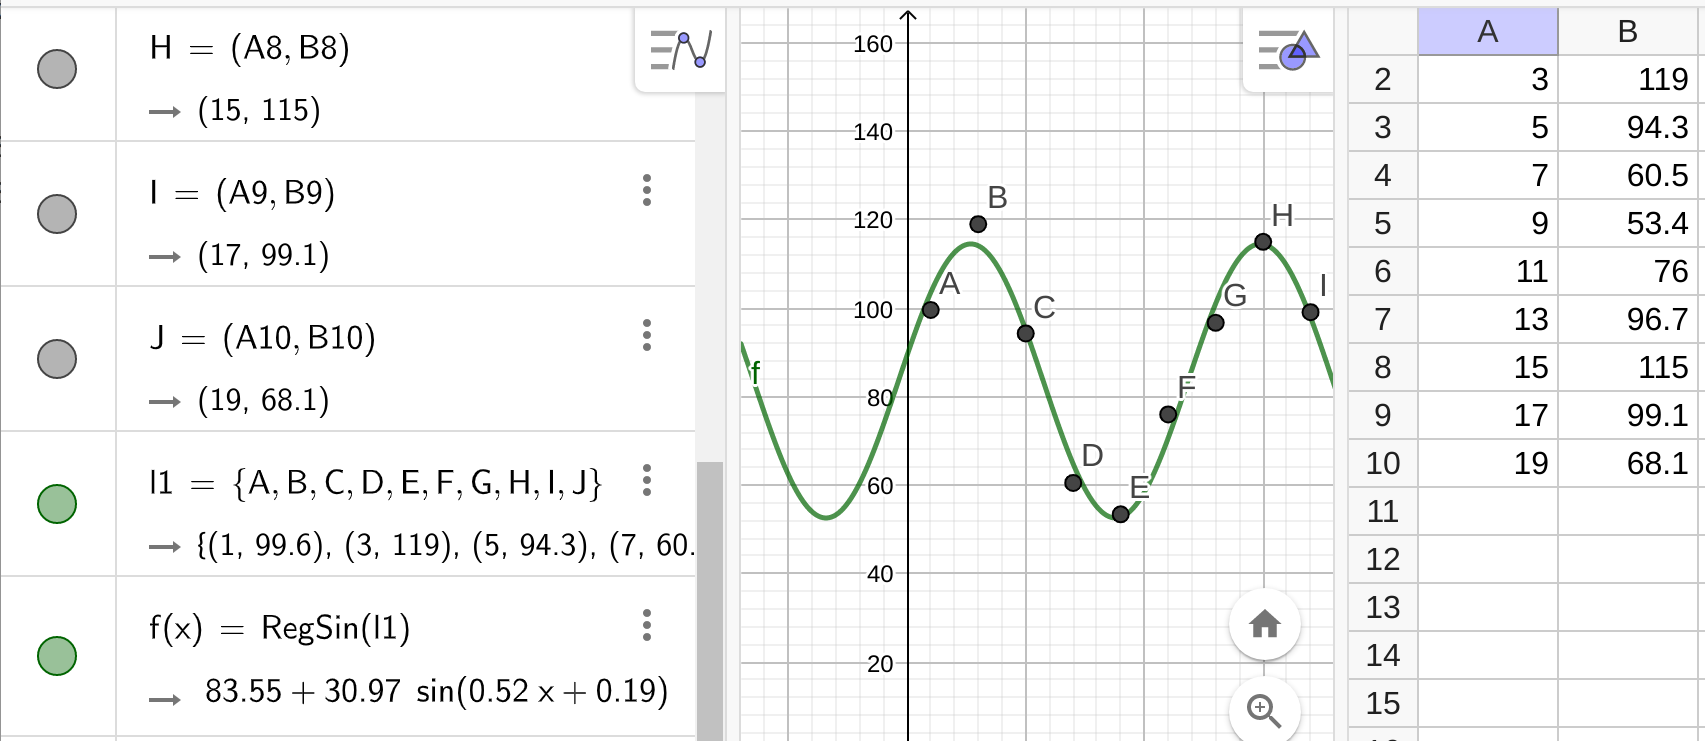
\includegraphics[scale=0.2]{opg1a}
\end{figure}
\item Den største økningen i vannstand skjer når $ f'(x) $ når sitt toppunkt. For å finne ekstremalpunkt 25. april må vi søke på intervallet $ [24, 48] $. Finner da at $ f'(x) $ har toppunkt når $ x\approx36.5 $, altså ca. kl. $ 12 $ den dagen. 
\begin{figure}
	\centering
	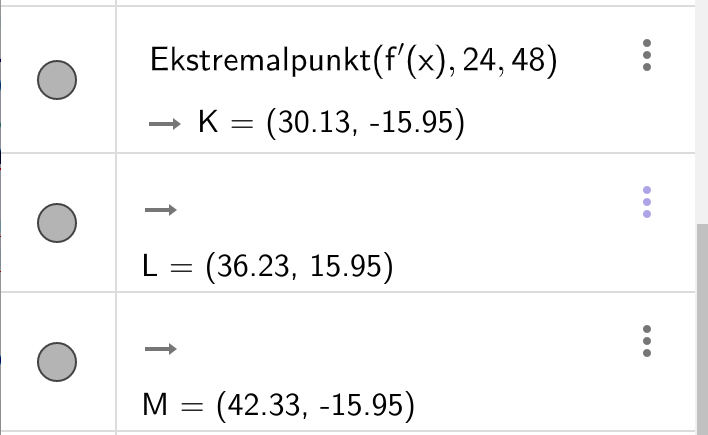
\includegraphics[scale=0.2]{opg1b}
\end{figure}
\item Av inspeksjon av grafen ser vi at vannstanden er synkende i det siste skjæringspunktet mellom $ f $ og linja $ y=90 $ på intervallet $ [24, 48] $. Dette skjæringspunktet er når $ x=\approx 42 $, som betyr at båten må slepes senest når $ x\approx40 $, altså kl. 16:00.
 \begin{figure}
 	\centering
 	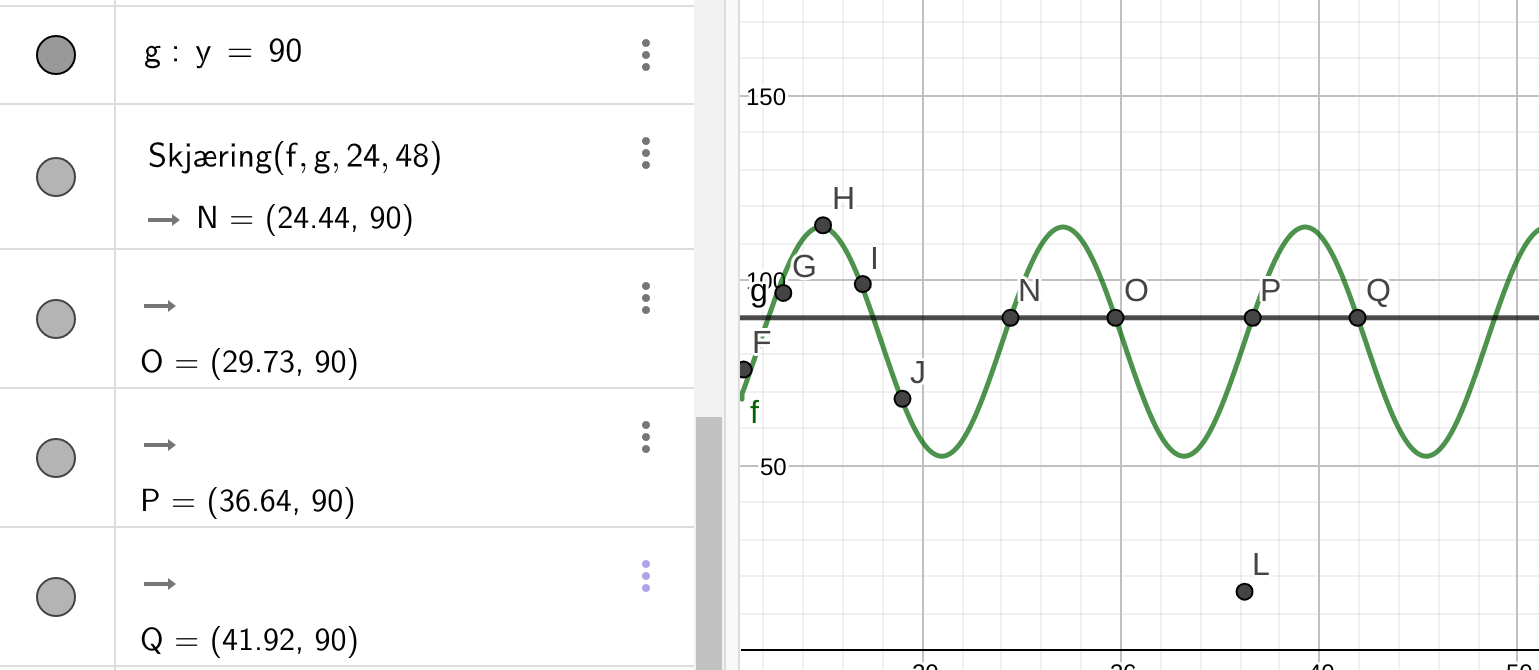
\includegraphics[scale=0.2]{opg1c}
 \end{figure}
}
\subsection*{Oppgave 2}
\abc{
\item 
Det ytre pentagonet i figur $ n $ har $ 5(n-1) $ kuler. Da det ytre pentagonet er det eneste som skiller figur $ n $ og figur $ n-1 $, har vi at
\[ P_{n}=5(n-1)+P_{n-1} \]
\item\phantom{a} \python{opg2.py}
\item Vi har at
\alg{
P_1&=1=1+5\cdot0\\
P_2&=6=1+5\cdot1  \\
P_3&=16=1+5\cdot1 + 5\cdot2=1+5(1+2) \\
P_4&=31=1+5\cdot 1+5\cdot2+5\cdot3=1+5(1+2+3) \\
P_5&=51=1+ 5\cdot1+5\cdot2+5\cdot3+5\cdot4=1+5(1+2+3+4)
}
Av dette ser vi at $ P_n=1+S_{n-1} $, hvor $ S_{n-1} $ er summen av de $ n-1 $ første naturlige tallene. $ S_{n-1}=\frac{n(n-1)}{2} $, og dermed er
\[ P_n=1+\frac{5n(n-1)}{2} \]
Det er åpenbart at formelen stemmer for $ n=1 $. Videre må vi, av den rekursive formelen, ha at
\begin{equation}\label{opg2i}
	P_{n+1}=5(n+1-1)+P_n = 1+\frac{5(n+1)n}{2}
\end{equation}
Vi antar at den eksplisitte formelen gjelder for $ P_n $, da kan vi skrive
\begin{align}
	P_{n+1}&=5n+P_n \nonumber \\
	&= 5n+1+\frac{5n(n-1)}{2} \nonumber \\
	&= 1+\frac{5n\cdot2+5n(n-1)}{2} \nonumber \\
	&= 1+\frac{5n(2+n-1)}{2} \nonumber\\
	&= 1+\frac{5n(n+1)}{2} \label{opg2ii}
\end{align}
\eqref{opg2i} samsvarer med \eqref{opg2ii}, og dermed er induksjonsbeviset fullført.
}
\subsection*{Oppgave 3}
Vi definerer punktene $ A $, $ B $ og $ C $ ut ifra opplysningene om tønnen, og bruker deretter regresjon for å finne parabelen $ f $ som går gjennom disse tre punktene. Volumet tilsvarer volumet til omdreiningslegemet til $ f $ på intervallet $ [0, 75] $, som har verdi $ 437164.4 $. Da målene er gitt i cm er volumet $ 437.1644\enh{dm}^3\approx437\enh{l} $.

\subsection*{Oppgave 4}
\abc{
\item Vi har at
\alg{
	a &= \frac{31.2-18.2}{2} = 7.5 \\
	d &= \frac{31.2+18.2}{2} = 24.7
}
Ut ifra oppgavebeskrivelsen antar vi det menes at $ M $ har en periode lik $ 24 $. Da er
\alg{
	c &= \frac{2\pi}{24}
}
\item I CAS-celle 1 definerer vi $ f(x) $ til å være $ M(t) $ med ukjent $ k $, og løser deretter ligningen $ f(13)=27 $ (celle 2). Ved å inspisere grafen til $ f $ med fase $ k=-0.62 $ eller $ k=-3.04 $, ser vi at $ k=-3.04 $ passer best til beskrivelsen i oppgaveteksten. Med denne verdien definerer vi $ M(t) $ i celle 3, og løser ligningen $ M=27 $ (celle 4). Da finner vi at det andre tidspunktet luftforurensingen har verdi 27 er når $ t=22.23 $, altså ca. kl. 22:10.
\begin{figure}
	\centering
	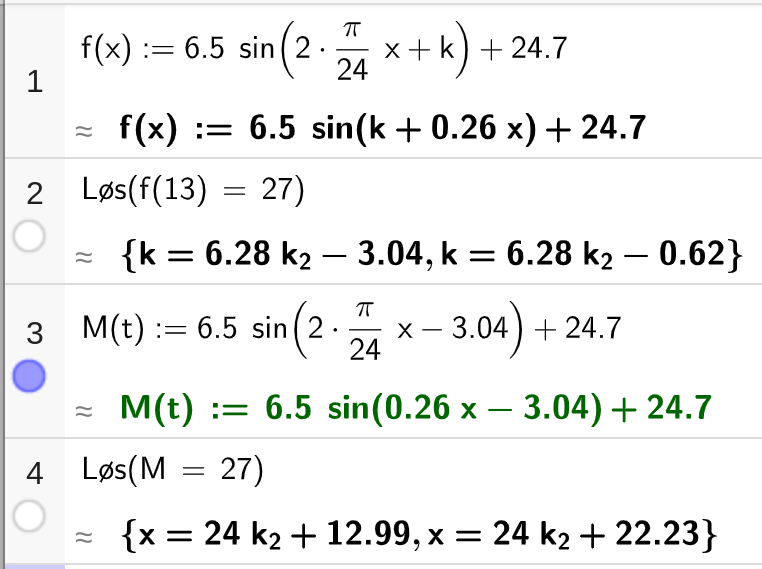
\includegraphics[scale=0.3]{opg4}
\end{figure}
}

\subsection*{Oppgave 5}
\abc{
\item Vi definerer $ r_1(t) $ som $ r(t) $ i CAS (celle 1). Skal en tangent til $ C $ være parallell med $ xy $-planet, må $ z $-kordinaten til $ r'(t) $ (celle 2) være 0. På intervallet $ (0, 2\pi) $ er $ \sin t=0 $ bare når $ t=\pi $, og dermed er punktet vi søker $ r(\pi)=(0, \pi, -1) $.
\item Se celle 3.
\item Cosiniusverdien til vinkelen mellom et plan med normalvektor $ \vec{n} $ og en linje med retningsvektor $ \vec{a} $ er gitt som
\[ \frac{|\vec{n}\cdot\vec{a}|}{|\vec{n}||\vec{a}|} \]
I celle 4 finner vi en normalvektor til smygplanet. $ [0, 1, 0] $ er en retningsvektor (med lengde 1) for $ y $-aksen. Da $ \cos^2 t+\sin^2 t=1 $ for alle $ t $, får vi av celle 5 at cosinusverdien er $ \frac{1}{\sqrt{2}} $ for alle $ t $. Dette betyr at vinkelen er $ 45^\circ $.
\begin{figure}
	\centering
	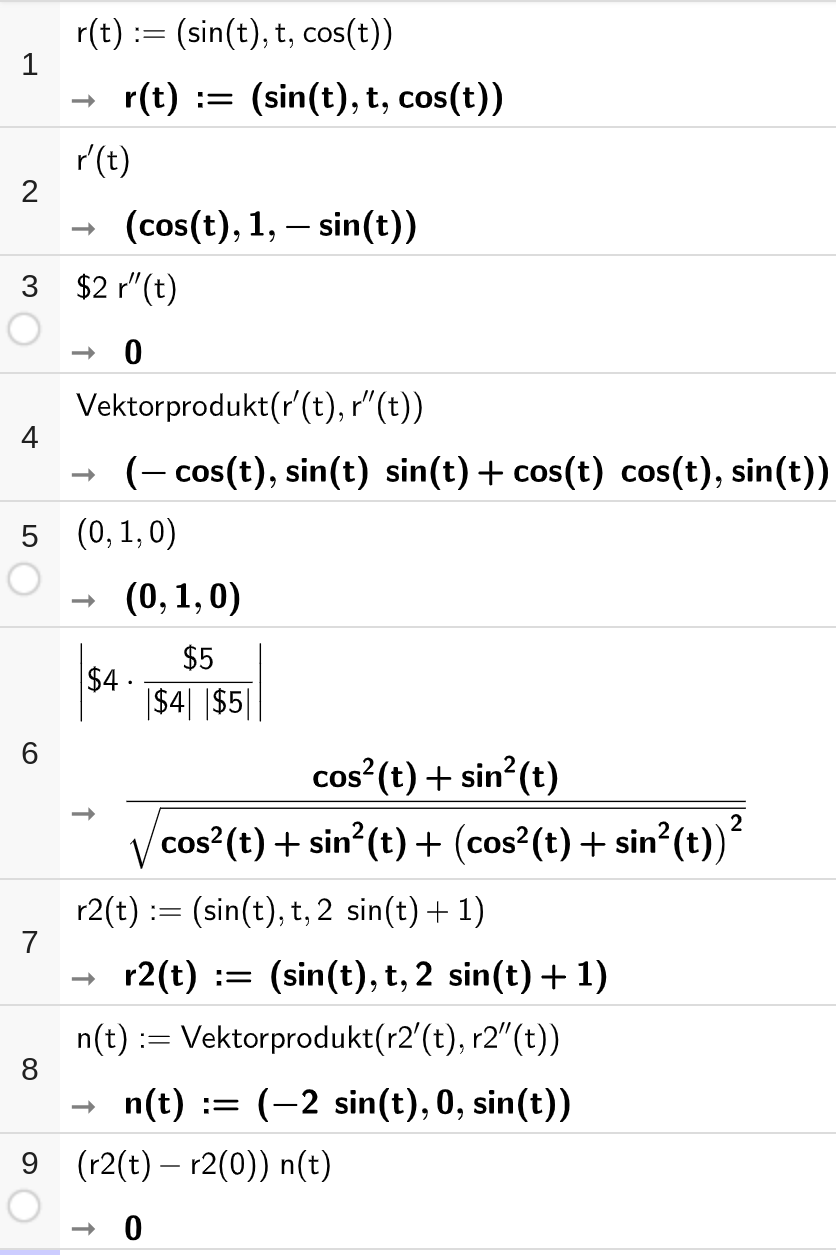
\includegraphics[scale=0.3]{opg5}
\end{figure}
\item For en vektorfunksjon
}

\end{document}